\chapter{Ergebnisse}
\subsection{Ergebnisse verschiedener Diskretisierungen }
\subsubsection{Allgemeine Darstellung der Ergebnisse}
Die hier tabellarisch präsentierten Ergebnisse werden in den folgenden
Kapiteln näher erleutert.



\begin{center}
\begin{minipage}{17cm}
\captionof{table}[RDM{}-Ergebnisse für die Dipolorientierungen cranial,
dorsal und sinistral in Abhängigkeit von der Diskretisierung der
inneren BEM{}-Schichten.]{RDM-Ergebnisse für die Dipolorientierungen
cranial, dorsal und sinistral in Abhängigkeit von der Diskretisierung
der inneren BEM-Schichten. }
\label{seq:refTable1}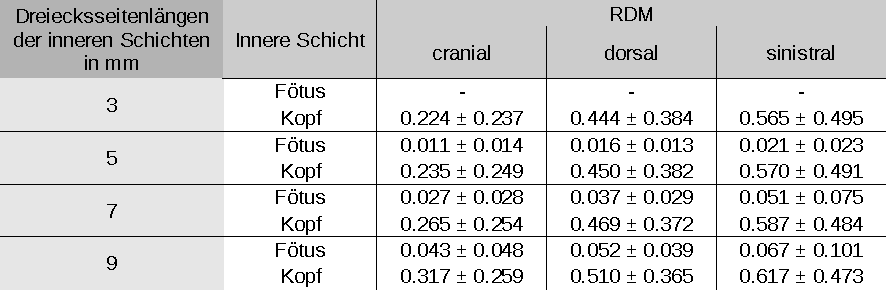
\includegraphics[width=15.035cm,height=4.957cm]{BA-img/BA-img14.pdf}\end{minipage}
\end{center}


\begin{center}
\begin{minipage}{17cm}
\captionof{table}[MAG{}-Ergebnisse für die Dipolorientierungen cranial,
dorsal und sinistral in Abhängigkeit von der Diskretisierung der
inneren BEM{}-Schichten.]{MAG-Ergebnisse für die Dipolorientierungen
cranial, dorsal und sinistral in Abhängigkeit von der Diskretisierung
der inneren BEM-Schichten. }
\label{seq:refTable2}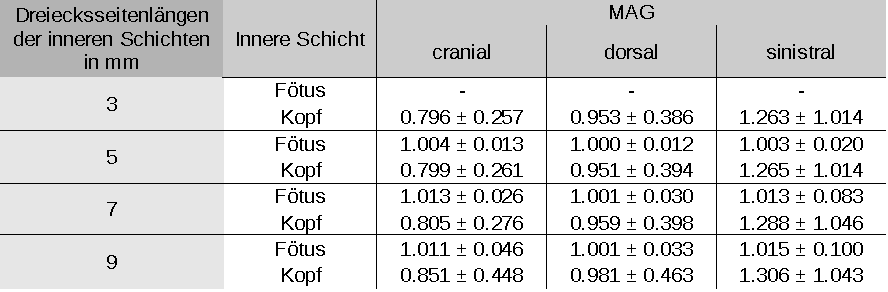
\includegraphics[width=15.035cm,height=4.957cm]{BA-img/BA-img15.pdf}\end{minipage}
\end{center}


\begin{center}
\begin{minipage}{17cm}
\captionof{table}[Winkelabweichungen für die Dipolorientierungen
cranial, dorsal und sinistral in Abhängigkeit von der Diskretisierung
der inneren BEM{}-Schichten.]{Winkelabweichungen für die
Dipolorientierungen cranial, dorsal und sinistral in Abhängigkeit von
der Diskretisierung der inneren BEM-Schichten. }
\label{seq:refTable3}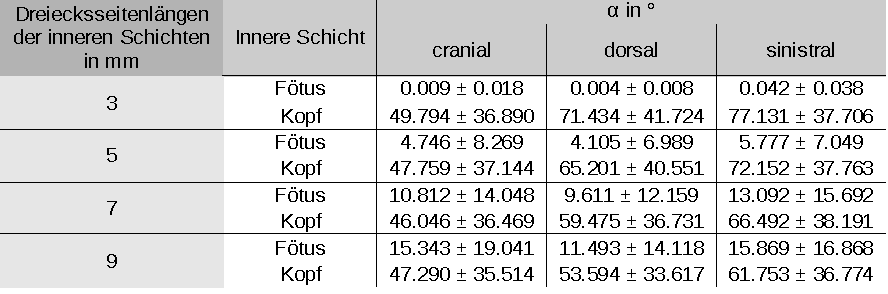
\includegraphics[width=15.035cm,height=4.957cm]{BA-img/BA-img16.pdf}\end{minipage}
\end{center}


\begin{center}
\begin{minipage}{17cm}
\captionof{table}[Amplitudenfaktoren für die rekonstruierten Dipole mit
cranialer, dorsaler und sinistraler Orientierung \ in Abhängigkeit von
der Diskretisierung der inneren BEM{}-Schichten.]{Amplitudenfaktoren
für die rekonstruierten Dipole mit cranialer, dorsaler und sinistraler
Orientierung  in Abhängigkeit von der Diskretisierung der inneren
BEM-Schichten. }
\label{seq:refTable4}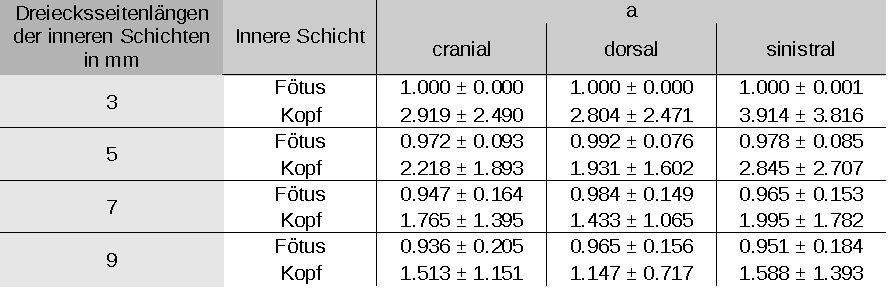
\includegraphics[width=15.035cm,height=4.957cm]{BA-img/BA-img17.pdf}\end{minipage}
\end{center}
\subsubsection{Vergleich der Diskretisierungseinflüsse auf direktes und
inverses Problem bei der Segmentierung des Fötus (BEM-Modelle 1 bis 3)}
\paragraph{Exaktheit der Lösung des direkten Problems
(Vorwärtssimulation)}
Beim Vergleich der \textit{RDM}{}-Ergebnisse für verschiedene
Randelementediskretisierungen ausgehend von der Segmentierung des
Fötus, ist zu sehen (\tablename~\ref{seq:refTable1}), dass sowohl die
\textit{RDM}{}-Mittelwerte als auch deren Standardabweichungen mit den
Diskretisierungsstufen ansteigen. Im Mittel liegen die \textit{RDMs
}für die Dipolorientierungen cranial und dorsal unter 0.05, bei den
Modellen 1 und 2 sogar unter der Schwelle 0.03. Die \textit{RDMs} und
damit die Topologieabweichungen der Magnetfelder für eine
Quellenorientierung nach links (sinistral) sind höher als die für
craniale oder dorsale Quellenorientierungen
(\tablename~\ref{seq:refTable1}).

Die MAG-Werte der Modelle 1 bis 3 liegen im Mittel zwischen 1 und 1.02,
wobei deren Standardabweichungen mit der Größe der Dreiecksseitenlängen
in den Modellen steigen, wie in \tablename~\ref{seq:refTable2}
aufgelistet.

\paragraph[Exaktheit der Rekonstruktionsergebnisse]{Exaktheit der
Rekonstruktionsergebnisse}
Die Winkelabweichungen der rekonstruierten Dipolorientierungen zu den
Referenzorientierungen (cranial, dorsal oder sinistral) und deren
Standardabweichungen steigen mit gröber werdender Diskretisierung der
Randelemente in den Modellen 1 bis 3 (\tablename~\ref{seq:refTable3}).

\tablename~\ref{seq:refTable4} zeigt, dass die rekonstruierten
Dipolstärken bei steigender Dreiecksseitenlänge in den BEM-Modellen 1
bis 3 kleiner werden, während ihre Standardabweichungen zunehmen.

\subsubsection{Vergleich der Diskretisierungseinflüsse auf direktes und
inverses Problem bei der Segmentierung des Fötuskopfes (BEM-Modelle 4
bis 7)}
\paragraph{Exaktheit der Lösung des direkten Problems
(Vorwärtssimulation)}
Die Topologieabweichungen von den Referenzfeldern, gemessenen in
\textit{RDM} und dargestellt in \tablename~\ref{seq:refTable1}, sind
bei den Modellen 4 bis 7 näherungsweise konstant für die jeweilige
Dipolorientierung. Bei sinistral ausgerichteten Dipolen sind die
Abweichungen im Mittel etwas höher als bei dorsal ausgerichteten und
die Abweichungen der Felder von cranial gerichteten Dipolen sind nur
ca. halb so groß wie die von dorsal gerichteten.

Wird das BEM-Modell 4 (Modell mit höherer örtlicher Auflösung in der
Diskretisierung verglichen mit den anderen Modellen ausgehend von der
Segmentierung des Fötuskopfes) als Referenz verwendet, ergeben sich
deutlich niedrigere RDM-Mittelwerte und Standardabweichungen
(\tablename~\ref{seq:refTable5}).

Die RDM-Werte steigen mit den verwendeten Dreiecksseitenlängen in den
BEM-Modelle an.

Die Ergebnisse der Topologieabweichungen spiegeln sich in ähnlicher Form
auch in den Abweichungen der Amplituden, gemessen in \textit{MAG
}(\tablename~\ref{seq:refTable2}), wieder. Die Amplituden der Felder
von cranial gerichteten Dipolen sind in den Modellen 4 bis 7 etwas
kleiner (ca. 0.8) verglichen mit den Referenzfeldern, während die
Felder der sinistral gerichteten Dipole stärker als die der Referenz
sind (ca. 1.3fach). Dorsal gerichtete Dipole erzeugen in den Modellen 4
bis 6 mit \textit{MAG}{}-Ergebnissen von 0.95 bis 0.98.

Die Amplitudenfaktoren der Felder von Modell 5 bis 7 bezogen auf die
Felder von Modell 4, liegen bei ca. 1.0 bis 1.1
(\tablename~\ref{seq:refTable6}).



\begin{center}
\begin{minipage}{17cm}
\captionof{table}[RDM{}-Ergebnisse mit BEM{}-Modell 4 als Referenz für
die Modelle 5, 6 und 7 für die Dipolorientierungen cranial, dorsal und
sinistral in Abhängigkeit von der Diskretisierung der inneren
BEM{}-Schichten.]{RDM-Ergebnisse mit BEM-Modell 4 als Referenz für die
Modelle 5, 6 und 7 für die Dipolorientierungen cranial, dorsal und
sinistral in Abhängigkeit von der Diskretisierung der inneren
BEM-Schichten. }
\label{seq:refTable5}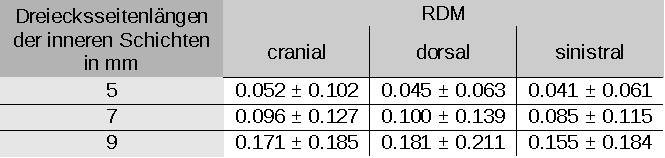
\includegraphics[width=11.269cm,height=2.699cm]{BA-img/BA-img18.pdf}\end{minipage}
\end{center}


\begin{center}
\begin{minipage}{17cm}
\captionof{table}[MAG{}-Ergebnisse mit BEM{}-Modell 4 als Referenz für
die Modelle 5, 6 und 7 für die Dipolorientierungen cranial, dorsal und
sinistral in Abhängigkeit von der Diskretisierung der inneren
BEM{}-Schichten.]{MAG-Ergebnisse mit BEM-Modell 4 als Referenz für die
Modelle 5, 6 und 7 für die Dipolorientierungen cranial, dorsal und
sinistral in Abhängigkeit von der Diskretisierung der inneren
BEM-Schichten. }
\label{seq:refTable6}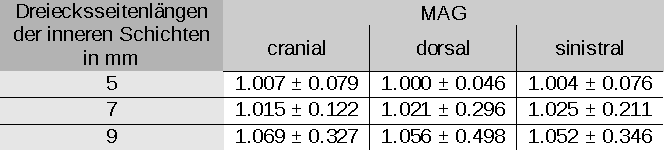
\includegraphics[width=11.269cm,height=2.593cm]{BA-img/BA-img19.pdf}\end{minipage}
\end{center}
\paragraph{Exaktheit der Rekonstruktionsergebnisse}
In \tablename~\ref{seq:refTable3} ist zu sehen, dass die Orientierungen
der rekonstruierten Dipole bei Verwendung der Modelle, die vom
segmentierten Fötuskopf entstanden, sehr stark (über 40° bis fast 80°)
von den ursprünglichen Orientierungen (cranial, dorsal oder sinistral)
abweichen.

Die rekonstruierten Dipolstärken sind bei Verwendung der Modelle 4 bis 7
größer als die definierten Dipole in der Vorwärtsrechnung. Eine
Dipolorientierung nach links (sinistral) hat bei diesen Modellen eine
größere Amplitude der rekonstruierten Quellen zur Folge (bis zum
4fachen der Referenzamplituden) als die Orientierungen cranial und
dorsal (\tablename~\ref{seq:refTable4}).

Mit dem Anstieg der Größe der Dreiecksseitenlängen in den BEM-Modellen,
nehmen die Abweichungen der rekonstruierten Orientierungen und Stärken
der Dipole von den idealen Ergebnissen ab.

\subsection{Vergleich der zwei Segmentierungsgrundlagen (Fötus und
Fötuskopf)}
\subsubsection{Exaktheit der Lösung des direkten Problems
(Vorwärtssimulation)}
Beim Vergleich von Fötus- und Kopfsegmentierung als Grundlage für das
BEM-Modell, in \tablename~\ref{seq:refTable1}, ist ein deutlicher
Unterschied im RDM-Level erkennbar, dabei sind die RDM-Mittelwerte und
Standardabweichungen des Modells von der Kopfsegmentierung in allen
Auflösungen ca. um eine 10er Potenz höher.

Die Amplitudenfaktoren der Felder von Modellen der Kopfsegmentierung
weichen deutlich mehr von 1 ab und haben größere Standardabweichungen
als die der Felder von Modellen der Fötussegmentierung
(\tablename~\ref{seq:refTable2}).

\subsubsection{Exaktheit der Rekonstruktionsergebnisse}
Beim Vergleich der entstehenden Orientierungsdifferenzen durch die
Verwendung verschiedener Segmentierungen für die BEM-Modellerstellung,
in \tablename~\ref{seq:refTable3}, wird deutlich, dass die
Segmentierung des Fötuskopfes als Grundlage große Abweichungen (bis
80°) zur Folge hat, während die Segmentierung des gesamten Fötus eine
Grundlage bietet, welche kleine Orientierungsdifferenzen (bis 15°) bei
der Quellenrekonstruktion aufweist.

Die Amplitudenfaktoren und Standardabweichungen der rekonstruierten
Dipole in Modellen der Kopfsegmentierung sind größer als die der
Quellen in Modellen der Fötussegmentierung, welche nahe bei 1 liegen
(\tablename~\ref{seq:refTable4}). Eine Abhängigkeit von der
Diskretisierung ist nicht direkt erkennbar.

\subsection{Vergleich verschiedener Vernixschichtdicken (Modelle 8 und
9)}
\subsubsection{Exaktheit der Lösung des direkten Problems
(Vorwärtssimulation)}


\begin{center}
\begin{minipage}{17cm}
\captionof{table}{MAG-Ergebnisse für die Dipolorientierungen cranial,
dorsal und sinistral in Abhängigkeit von der Schichtdicke der Vernix
caseosa.}
\label{seq:refTable7}
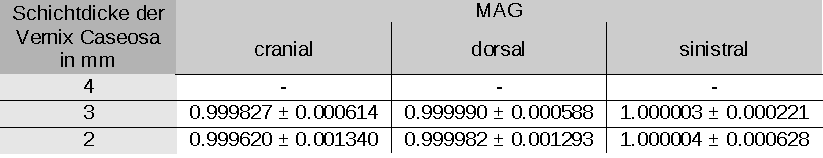
\includegraphics[width=13.951cm,height=2.699cm]{BA-img/BA-img20.pdf}\end{minipage}
\end{center}


\begin{center}
\begin{minipage}{17cm}
\captionof{table}{RDM-Ergebnisse für die Dipolorientierungen cranial,
dorsal und sinistral in Abhängigkeit von der Schichtdicke der Vernix
caseosa.}
\label{seq:refTable8}
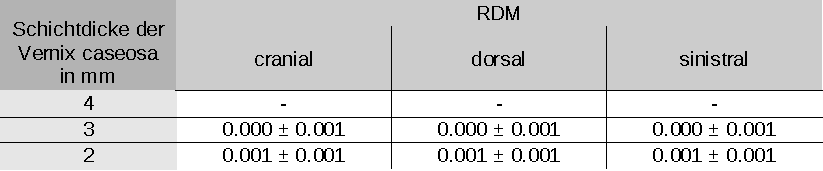
\includegraphics[width=13.951cm,height=2.909cm]{BA-img/BA-img21.pdf}\end{minipage}
\end{center}
Die RDM- und MAG-Ergebnisse für BEM-Modelle mit einer kleineren
Vernixschichtdicke als im Referenzmodell (BEM-Modell 0), wie in
\tablename~\ref{seq:refTable7} und \tablename~\ref{seq:refTable8}
angegeben, weichen sowohl bei einer Reduktion der Vernixschichtdicke um
1mm bzw. $\frac{1}{4}$ als auch um 2mm bzw. $\frac{1}{2}$ nur marginal
von den minimalen Fehlern (MAG=1 und RDM=0) ab. Die Abweichungen der
Felder von sinistral gerichteten Dipolen sind hier kleiner als die der
Felder von cranial oder dorsal gerichteten Dipolen. 

\subsubsection[Exaktheit der Rekonstruktionsergebnisse]{Exaktheit der
Rekonstruktionsergebnisse}


\begin{center}
\begin{minipage}{17cm}
\captionof{table}{Winkelabweichungen für die Dipolorientierungen
cranial, dorsal und sinistral in Abhängigkeit von der Diskretisierung
der Schichtdicke der Vernix caseosa.}
\label{seq:refTable9}
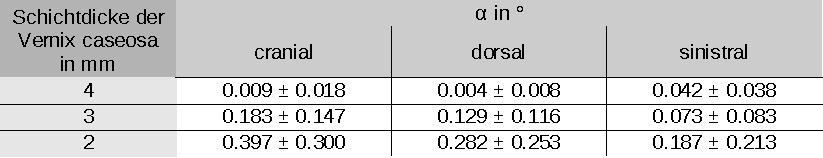
\includegraphics[width=13.951cm,height=2.699cm]{BA-img/BA-img22.pdf}\end{minipage}
\end{center}


\begin{center}
\begin{minipage}{17cm}
\captionof{table}[Amplitudenfaktoren für die rekonstruierten Dipole mit
cranialer, dorsaler und sinistraler Orientierung \ in Abhängigkeit von
der Diskretisierung der inneren BEM{}-Schichten.]{Amplitudenfaktoren
für die rekonstruierten Dipole mit cranialer, dorsaler und sinistraler
Orientierung  in Abhängigkeit von der Diskretisierung der inneren
BEM-Schichten.}
\label{seq:refTable10}
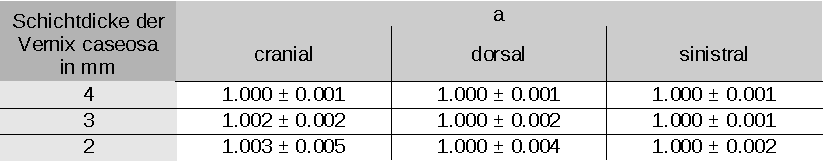
\includegraphics[width=13.951cm,height=2.752cm]{BA-img/BA-img23.pdf}\end{minipage}
\end{center}
In \tablename~\ref{seq:refTable9} ist zu sehen, dass die Orientierungen
der rekonstruierten Dipole bei Verwendung des Modells mit einer
Vernixschichtdicke von 3mm kaum (weniger als 1°) von den ursprünglichen
Orientierungen (cranial, dorsal oder sinistral) abweichen. Das gleiche
gilt für die Verwendung des Modells mit einer Vernixschichtdicke von
2mm, wobei ein Anstieg des Orientierungsfehlers mit sinkender
Vernixschichtdicke erkennbar ist.

Die Amplitudenfaktoren der rekonstruierten Dipole für BEM-Modelle mit
einer kleineren Vernixschichtdicke als 4mm, wie sie im Referenzmodell
(BEM-Modell 0) verwendet wurde, zeigen
(\tablename~\ref{seq:refTable10}), dass eine kleinere
Vernixschichtdicke mit einem Anstieg der rekonstruierten Dipolstärken
verbunden ist.

Wie bei den Ergebnissen der Lösung des direkten Problems sind die
Abweichungen von den idealen Lösungen auch beim inversen Problem bei
sinistral gerichteten Dipolen kleiner als bei cranial oder dorsal
gerichteten Dipolen (\tablename~\ref{seq:refTable9} und
\tablename~\ref{seq:refTable10}).

